\documentclass[border=6pt]{standalone}
\usepackage{tikz}
\usetikzlibrary{arrows.meta,positioning,calc,shapes.geometric,fit,backgrounds,patterns,matrix,decorations.pathreplacing}
\begin{document}
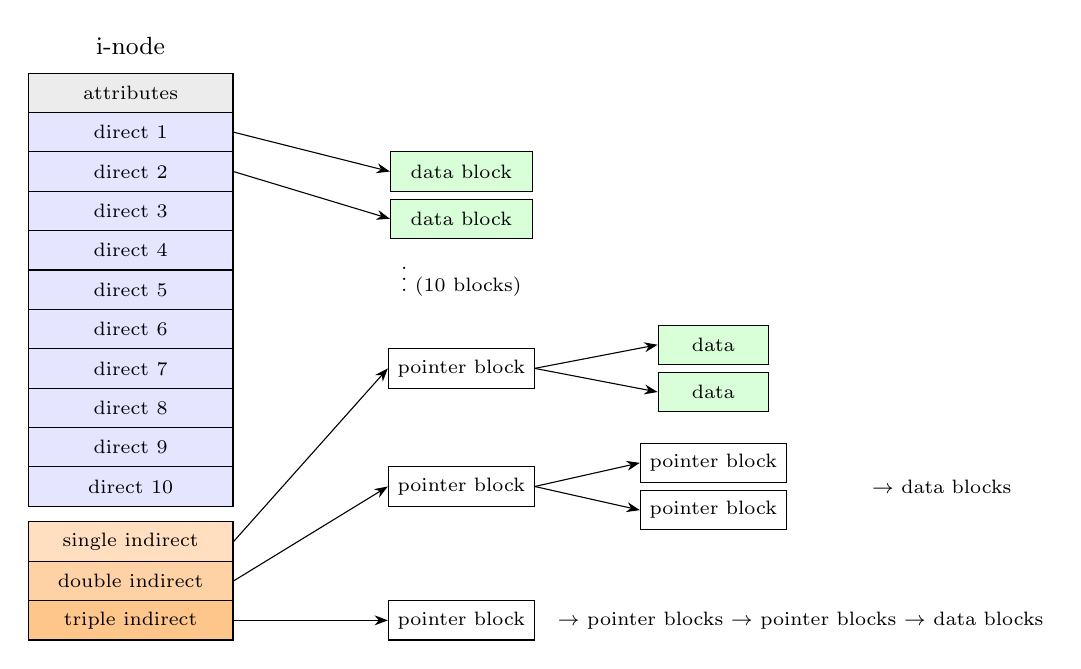
\begin{tikzpicture}[>=Stealth,font=\small]
\tikzstyle{c}=[draw,minimum height=0.5cm,minimum width=2.6cm,font=\scriptsize]
\node[font=\small] at (0,0.6) {i-node};
\node[c,fill=gray!15] at (0,0) {attributes};
\foreach \i in {1,...,10} \node[c,fill=blue!10] (d\i) at (0,-\i*0.5) {direct \i};
\node[c,fill=orange!25] (s) at (0,-5.7) {single indirect};
\node[c,fill=orange!35] (d) at (0,-6.2) {double indirect};
\node[c,fill=orange!45] (t) at (0,-6.7) {triple indirect};
\node[c,fill=green!15,minimum width=1.8cm] (b1) at (4.2,-1.0) {data block};
\node[c,fill=green!15,minimum width=1.8cm] (b2) at (4.2,-1.6) {data block};
\draw[->] (d1.east) -- (b1.west); \draw[->] (d2.east) -- (b2.west);
\node[font=\scriptsize] at (4.2,-2.3) {$\vdots$ (10 blocks)};
\node[c,minimum width=1.8cm] (i1) at (4.2,-3.5) {pointer block}; \draw[->] (s.east) -- (i1.west);
\node[c,fill=green!15,minimum width=1.4cm] (e1) at (7.4,-3.2) {data}; \node[c,fill=green!15,minimum width=1.4cm] (e2) at (7.4,-3.8) {data};
\draw[->] (i1.east) -- (e1.west); \draw[->] (i1.east) -- (e2.west);
\node[c,minimum width=1.8cm] (i2) at (4.2,-5.0) {pointer block}; \draw[->] (d.east) -- (i2.west);
\node[c,minimum width=1.8cm] (j1) at (7.4,-4.7) {pointer block}; \node[c,minimum width=1.8cm] (j2) at (7.4,-5.3) {pointer block};
\draw[->] (i2.east) -- (j1.west); \draw[->] (i2.east) -- (j2.west);
\node[font=\scriptsize] at (10.3,-5.0) {$\to$ data blocks};
\node[c,minimum width=1.8cm] (k) at (4.2,-6.7) {pointer block}; \draw[->] (t.east) -- (k.west);
\node[font=\scriptsize,anchor=west] at (5.3,-6.7) {$\to$ pointer blocks $\to$ pointer blocks $\to$ data blocks};
\end{tikzpicture}
\end{document}
